\section{Diseño}

\subsection{Diseño de las clases de la Arquitectura}

La arquitectura de implementación del sistema de generación de terreno procedural en Unity se compone de varios componentes interconectados que colaboran para lograr la generación y representación eficiente del terreno del juego. A continuación, se detallan las clases y su papel en el proceso de generación de terreno. Los componentes que se seleccionaron en la fase Análisis ahora se han agrupado para generar dos subsistemas para la generación de alturas y la generación del terreno en sí.

\subsubsection{Generación de alutras}

Los Jobs son unidades de trabajo paralelo que se utilizan para tareas intensivas en la CPU, como la generación de terreno y la erosión.

\begin{itemize}
    
    \item \textbf{Noise}: proporciona métodos para generar ruido Perlin, Simplex y Voronoi, que se utilizan para crear el mapa de altura del terreno.
    \begin{itemize}
        \item Genera ruido 2D y 3D utilizando algoritmos de ruido Perlin, Simplex y Voronoi.
        \item Permite configurar parámetros como la escala, octavas y persistencia para controlar la apariencia del terreno.
        \item Utiliza Unity Jobs y la biblioteca Burst para la generación eficiente de ruido.
    \end{itemize}

    \item \textbf{ErosionJob}: un Job que aplica algoritmos de erosión al terreno generado.
    \begin{itemize}
        \item Calcula la erosión térmica en cada punto del terreno, suavizando las pendientes y mejorando la autenticidad del terreno.
        \item Trabaja en conjunto con el mapa de altura y la configuración de erosión para lograr resultados realistas.
        \item Ayuda a simular procesos de erosión realistas en el terreno.
    \end{itemize}

    \item \textbf{MapGeneratorJob}: un Job que se utiliza para generar el mapa de altura del terreno.
    \begin{itemize}
        \item Utiliza algoritmos de ruido y configuración de generación para crear el mapa de altura del terreno.
        \item Paraleliza la generación para un rendimiento eficiente.
    \end{itemize}
    
\end{itemize}

\subsubsection{Generación y gestión del Terreno}

Los Generadores del Terreno gestionan la creación y visualización de partes del terreno (chunks) en el mundo del juego. Se aseguran de que solo se carguen los chunks visibles y que se utilicen niveles de detalle (LOD) para optimizar el rendimiento.

\begin{itemize}
    \item \textbf{EndlessTerrain}: es responsable de la gestión de los chunks de terreno infinito. Controla la carga y descarga dinámica de los chunks en función de la posición del jugador y los niveles de detalle (LOD).
    \begin{itemize}
        \item Actualiza la posición del jugador y determina qué chunks deben cargarse o descargarse.
        \item Utiliza un conjunto de niveles de detalle (LOD) para optimizar la calidad del terreno según la distancia al jugador.
        \item Almacena y gestiona un diccionario de chunks visibles en el mundo.
    \end{itemize}

    \item \textbf{TerrainChunk}: representa un chunk de terreno individual. Contiene la lógica para actualizar y visualizar un chunk, así como la gestión de LOD.
    \begin{itemize}
        \item Actualiza y visualiza un chunk de terreno en función de su posición y nivel de detalle (LOD).
        \item Almacena la malla del terreno y se encarga de su representación visual.
        \item Gestiona la solicitud y recepción de datos de mapa y malla mediante Jobs.
    \end{itemize}

    \item \textbf{MapGenerator}: se encarga de generar el mapa de altura del terreno, que define las elevaciones y depresiones del paisaje.
    \begin{itemize}
        \item Genera el mapa de altura utilizando algoritmos de ruido y otros métodos para crear un terreno detallado y realista.
        \item Controla parámetros como la escala, octavas y persistencia para ajustar la apariencia del terreno.
        \item Utiliza Unity Jobs y la biblioteca Burst para una generación eficiente de ruido.
    \end{itemize}

    \item \textbf{MeshGenerator}: se encarga de generar las mallas de los chunks de terreno.
    \begin{itemize}
        \item Genera las mallas de terreno de diferentes niveles de detalle (LOD) para su representación visual.
        \item Permite una transición suave entre mallas LOD para evitar artefactos visuales.
        \item Realiza solicitudes y recepciones de mallas de terreno mediante Jobs.
    \end{itemize}

    \item \textbf{MeshDataGeneratorJob}: un Job que genera datos de malla para los chunks de terreno.
    \begin{itemize}
        \item Calcula la geometría de la malla, incluyendo vértices, triángulos y coordenadas UV.
        \item Utiliza datos como el mapa de altura y la configuración de malla para generar la malla del terreno.
        \item Es parte integral del proceso de representación visual de los chunks de terreno.
    \end{itemize}

\end{itemize}

\subsubsection{Representación del Terreno}

Cómo ya se ha mencionado antes, son los propios chunks los que se encargan de gestionar su información y almacenan sus coordenadas de textura, no obstante, cuando se procesan los vértices para generar su altura, se crea un mapa paralelo que es el mapa de color, el cuál se convierte porsteriormente en una texura que servirá para la representación visual de los chunks.

\item \textbf{TextureGenerator}: se encarga de generar las texturas del terreno a partir del mapa de altura y otros datos.
\begin{itemize}
    \item Genera texturas utilizando datos como el mapa de altura y una paleta de colores.
    \item Permite personalizar la asignación de texturas a diferentes altitudes y características del terreno.
    \item Utiliza Unity Jobs para la generación de texturas eficiente.
\end{itemize}

\subsection{Diseño de la Arquitectura del Software}

\subsubsection{Diagrama de Clases}

En el siguiente diagrama de clases se detallan las relacioens entre los componentes del sistema.

\begin{figure}[H]
    \centering
    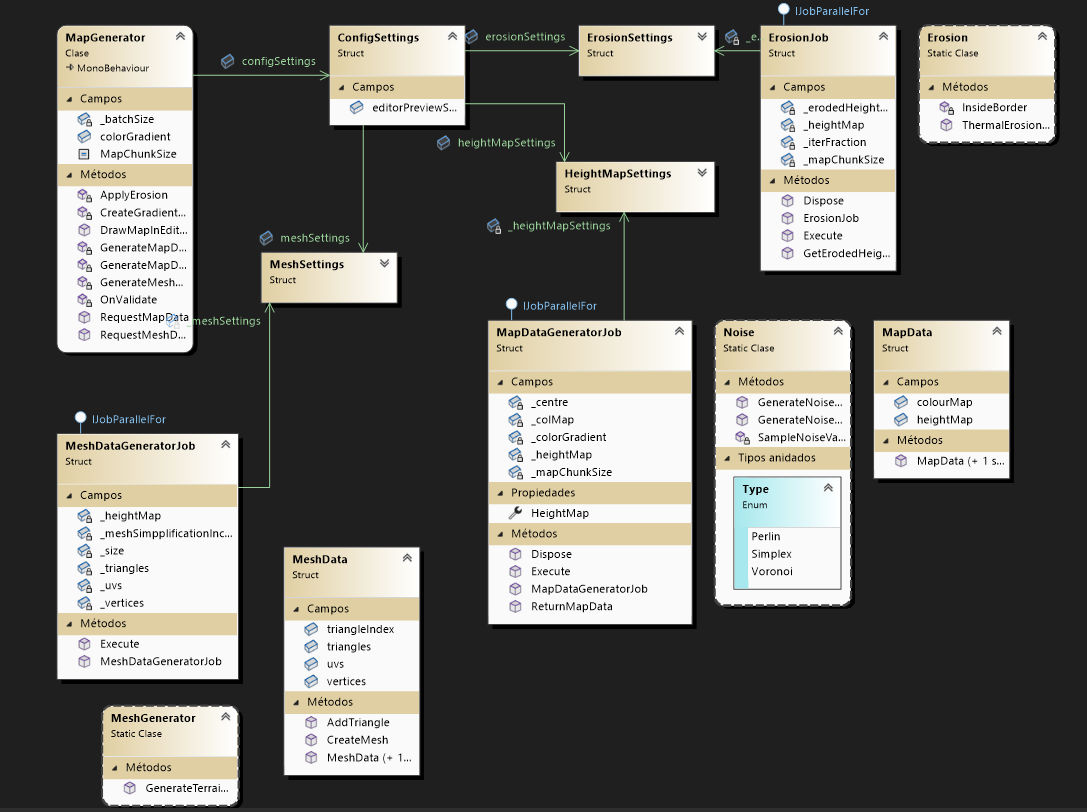
\includegraphics[width=1\textwidth]{img/diagrama de clases.png}
    \caption{Diagrama de Clases.}
\end{figure}


\subsection{Diseño Detallado}

% \subsubsection{Diagramas de Secuencia}
% Muestra los diagramas de secuencia que ilustran la interacción entre los componentes clave de tu sistema.

\subsubsection{Diagramas de Flujo}
Los siguientes diagramas de flujo representan los flujos de trabajo y procesos entre los distintos sistemas y componentes de la herramienta.

\begin{figure}[H]
    \centering
    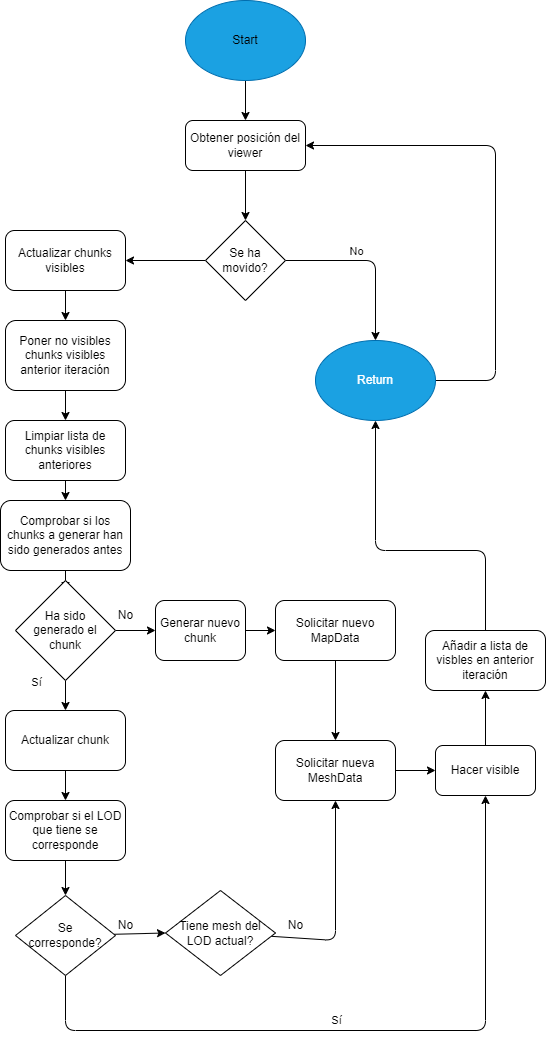
\includegraphics[width=0.65\textwidth]{img/FlowDiagramEndlessTerrain.png}
    \caption{Diagrama de Secuencia de Generación de Terreno desde el incio de EndlessTerrain.}
\end{figure}

\subsection{Desafíos y Decisiones de Diseño}

\subsubsection{Desafíos Técnicos}
Durante el diseño y desarrollo del proyecto, se enfrentaron varios desafíos técnicos significativos. Algunos de los desafíos más destacados incluyeron:

\begin{itemize}
    \item \textbf{Optimización de Rendimiento:} Lograr un rendimiento óptimo en la generación procedural de terrenos en tiempo real fue uno de los principales desafíos técnicos. Se implementó el Unity Job System y el Burst Compiler para abordar este desafío.
    
    \item \textbf{Generación Realista:} La generación de terrenos realistas y variados implicó la implementación de algoritmos de ruido Perlin, Simplex y Voronoi, así como la configuración adecuada de parámetros como escalas y octavas.
    
    \item \textbf{Erosión y Características Naturales:} Incorporar algoritmos de erosión para simular características naturales como ríos y cañones fue un desafío adicional.
    
    \item \textbf{Continuidad del terreno:} La continuidad del terreno nuevo que se genera, sin notar la transición entre partes de terreno generadas e integradas al terreno que ya había supuso otro tema técnico que hubo que resolver.
    
    \item \textbf{Corrección de borde en erosión:} Dado que a eroisón se reliza teniendo en cuenta las alturas de cada fragmento de terreno y equilibrándolas, porduce incosistencias con las partes de terreno. Resolver esto fue otro desafío.
    
    \item \textbf{Implementación de LOD:}  La inclusión de LOD supuso otro desafío ya que hubo que adaptar la estructura de como estaban modelados las partes de terreno que se generaban para añadir esta caracterísitca y mooficar la lógica de generación de terreno.
    
    \item \textbf{Paralelización de la creación del mapa de altura:} La creación de un mapa de alturas de manera paralela suspuso modificaciones de la manera tradicional de generación de mapas de altruas, que supuso tener que hacer adaptaciones.
     
    \item \textbf{Paralelización de la erosión del mapa de altura:} Del mismo modo que la creación de un mapa de alturas de manera paralela suspuso modificaciones de la manera tradicional, la erosión supuso una remodelación de la lógica no paralelizada con la que se idearon los algortimos de erosión que hubo que adaptar.
     
    \item \textbf{Paralelización de la creación del mapa de altura:} Por último, la configuración del array de vértices, uvs y triángulos de las meshes geenradas también debía hacerse de manera procedural por lo que al igual que en los dos casos anterior, hubo que estudiar la manera de hacerlo de manera óptima.

\end{itemize}

\subsubsection{Decisiones de Diseño}
Las decisiones de diseño desempeñaron un papel fundamental en la arquitectura y funcionalidad del proyecto. Algunas de las decisiones clave incluyeron:

\begin{itemize}
    \item \textbf{Uso del Unity Job System:} Se decidió utilizar el Unity Job System para la paralelización de tareas y optimizar la generación de terrenos, lo que resultó en un rendimiento mejorado.
    
    \item \textbf{Selección de Algoritmos de Ruido:} La elección de implementar algoritmos de ruido Perlin y Simplex permitió generar terrenos realistas y variados con una apariencia natural.
    
    \item \textbf{Erosión para Características Naturales:} La incorporación de algoritmos de erosión en el diseño permitió crear características naturales como ríos y cañones, mejorando la apariencia general del terreno.
    
    \item \textbf{Uso de LOD:} La incorporación de LOD al proyecto le añade un extra, que si bien no es una función a la cual se la haya aplicado paralelismo, es una característica más que extiende las capacidades de la herramienta permitiendo extender el terreno generable con menos costo que una generación no paralelizada total.
    
    \item \textbf{Elección de nave como explorador} La elección de elección de una nave como explorador de terreno se debió a que las irregularidades del terreno para terrenos escarpados podrían complicar la exploración, además de que con un sobrevuelo se pdoría ver mejor el rendimiento de la generació.
    
    \item \textbf{Configurabilidad:} Se diseñaron clases como `HeightMapSettings`, `MeshSettings`, y `ErosionSettings` para permitir la configuración flexible de varios parámetros del terreno. Los usuarios pueden ajustar la escala del ruido, la resolución de la malla y los efectos de erosión según sus necesidades.

\end{itemize}

\subsubsection{Consideraciones de Rendimiento}

Durante el diseño, se tuvieron en cuenta varias consideraciones de rendimiento para garantizar un sistema eficiente:

- \textbf{Optimización de Malla:} Se implementó una lógica de generación de malla eficiente que reduce la cantidad de vértices y triángulos en función del nivel de detalle, lo que mejora el rendimiento de renderizado.

- \textbf{Burst Compiler:} La utilización de la herramienta Burst Compiler permitió compilar el código C\# en código nativo altamente optimizado, mejorando aún más el rendimiento en la generación de terrenos.

- \textbf{Paralelización:} Aprovechar el paralelismo mediante el Unity Job System garantiza que la generación de terrenos se ejecute de manera eficiente en sistemas con múltiples núcleos de CPU.

% \subsection{Planificación de Desarrollo}

% \subsubsection{Cronograma de Desarrollo}

% El desarrollo de este proyecto se planificó en varias etapas, con hitos y fechas clave:

% - \textbf{Investigación y Diseño Inicial (Semanas 1-2):} En esta etapa, se realizó una investigación exhaustiva sobre algoritmos de generación de terrenos y se diseñó la arquitectura del sistema.

% - \textbf{Desarrollo de Componentes Clave (Semanas 3-4-5):} Se implementaron los componentes clave del sistema, como el `MapGenerator`, `MapDataGeneratorJob`, `MeshDataGeneratorJob`, y se realizaron pruebas de rendimiento.

% - \textbf{Integración de Erosión (Semanas 6-7):} Se trabajó en la integración de algoritmos de erosión y se afinaron los efectos de erosión.

% - \textbf{Optimización y Pruebas Finales (Semanas 7-8):} Se realizaron pruebas exhaustivas de rendimiento y se optimizó el código para garantizar una generación de terrenos eficiente.

% - \textbf{Documentación y Entrega (Semanas 9-10):} Se completó la documentación detallada del proyecto, incluyendo la memoria en LaTeX y la generación de diagramas.

% \subsection{Conclusión}

% En resumen, esta sección ha proporcionado una visión general del diseño de nuestro sistema, destacando las decisiones clave, las consideraciones de rendimiento y la planificación de desarrollo. A medida que avanzamos en el proyecto, seguiremos refinando y mejorando esta arquitectura para lograr nuestros objetivos. En las próximas secciones, nos centraremos en la implementación y las pruebas del sistema.
